\chapter{Graphs}
\chaplabel{graphs}

%\textbf{Warning to the Reader:} This chapter is still being actively
%developed, meaning that the code has not been thoroughly tested and/or
%the text has not be carefully proofread.

In this chapter, we study two representations of graphs and basic
algorithms on these representations.  

Mathematically, a \emph{(directed) graph} is a pair $G=(V,E)$ where
$V$ is a set of \emph{vertices} and $E$ is a set of ordered pairs
of vertices called \emph{edges}.  An edge #(i,j)# is \emph{directed}
from #i# to #j#;  #i# is called the \emph{source} of the edge and #j#
is called the \emph{target}.  A \emph{path} in $G$ is a sequence of
vertices $v_0,\ldots,v_k$ such that, for every $i\in\{1,\ldots,k\}$,
the edge $(v_{i-1},v_{i})$ is in $E$.  A path $v_0,\ldots,v_k$ is a
cycle if, additionally, the edge $(v_k,v_0)$ is in $E$.  A path (or
cycle) is \emph{simple} if all of its vertices are unique.  If there is
a path from some vertex $v_i$ to some vertex $v_j$ then we say that $v_j$
is \emph{reachable} from $v_i$.
An example of a graph is shown in \figref{graph}.

\begin{figure}
  \begin{center}
    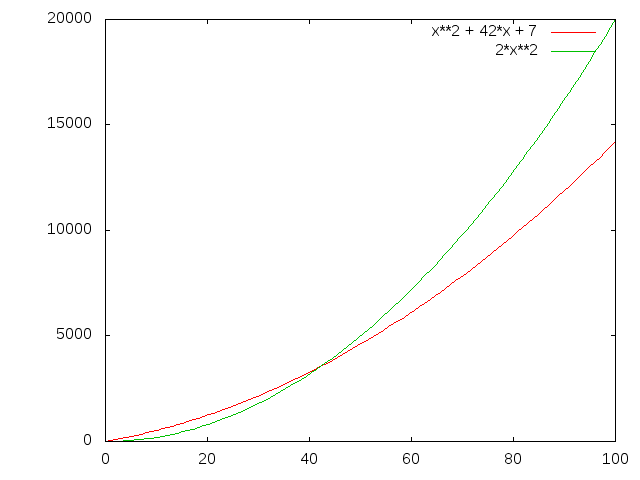
\includegraphics{figs/graph}
  \end{center}
  \caption{A graph with 12 vertices.  Vertices are drawn as numbered circles and edges are drawn as pointed curves pointing from source to target.}
  \figlabel{graph}
\end{figure}


Graphs have an enormous number of applications, due to their ability
to model so many phenomena. There are many obvious examples. Computer
networks can be modelled as graphs, with vertices corresponding to
computers and edges corresponding to (directed) communication links
between those computers.  Street networks can be modelled as graphs,
with vertices representing intersections and edges representing streets
joining consecutive intersections.

Less obvious examples occur as soon as we realize that graphs can model
any pairwise relationships within a set. For example, in a university
setting we might have a timetable conflict graph whose vertices represent
courses offered in the university and in which the edge #(i,j)# is present
if and only if there is at least one student that is taking both class
#i# and class #j#.  Thus, an edge indicates that the exam for class #i#
can not be scheduled at the same time as the exam for class #j#.

Throughout this section, we will use #n# to denote the number of vertices
of $G$ and #m# to denote the number of edges of $G$.  That is, $#n#=|V|$
and $#m#=|E|$. Furthermore, we will assume that $V=\{0,\ldots,#n#-1\}$.
Any other data that we would like to associate with the elements of $V$
can be stored in an array of length $#n#$.

Some typical operations performed on graphs are:
\begin{itemize}
  \item #addEdge(i,j)#: Add the edge $(#i#,#j#)$ to $E$.
  \item #removeEdge(i,j)#: Remove the edge $(#i#,#j#)$ from $E$.
  \item #hasEdge(i,j)#: Check if the edge $(#i#,#j#)\in E$ 
  \item #outEdges(i)#: Return a #List# of all integers $#j#$ such that
  $(#i#,#j#)\in E$
  \item #inEdges(i)#: Return a #List# of all integers $#j#$ such that
  $(#j#,#i#)\in E$
\end{itemize}

Note that these operations are not terribly difficult to implement
efficiently. For example, the first three operations can be implemented
directly by using a #USet#, so they can be implemented in constant
expected time using the hash tables discussed in \chapref{hashing}.
The last two operations can be implemented in constant time by storing,
for each vertex, a list of its adjacent vertices.

However, different applications of graphs have different performance
requirements for these operations and, ideally, we can use the simplest
implementation that satisfies all the application's requirements.
For this reason, we discuss two broad categories of graph representations.

\section{#AdjacencyMatrix#: Representing a Graph by a Matrix}
\seclabel{adjacency-matrix}

An \emph{adjacency matrix} is a way of representing an #n# vertex graph
$G=(V,E)$ by an $#n#\times#n#$ matrix, #a#, whose entries are boolean
values.
\codeimport{ods/AdjacencyMatrix.a.n.AdjacencyMatrix(n0)}

The matrix entry #a[i][j]# is defined as
\[  #a[i][j]#= 
    \begin{cases}
      #true# & \text{if $#(i,j)#\in E$} \\
      #false# & \text{otherwise}
    \end{cases}
\]
The adjacency matrix for the graph in \figref{graph} is
shown in \figref{graph-adj}.

With this representation, the #addEdge(i,j)#,
#removeEdge(i,j)#, and #hasEdge(i,j)# operations just
involve setting or reading the matrix entry #a[i][j]#:
\codeimport{ods/AdjacencyMatrix.addEdge(i,j).removeEdge(i,j).hasEdge(i,j)}
These operations clearly take constant time per operation.

\begin{figure}
  \begin{center}
    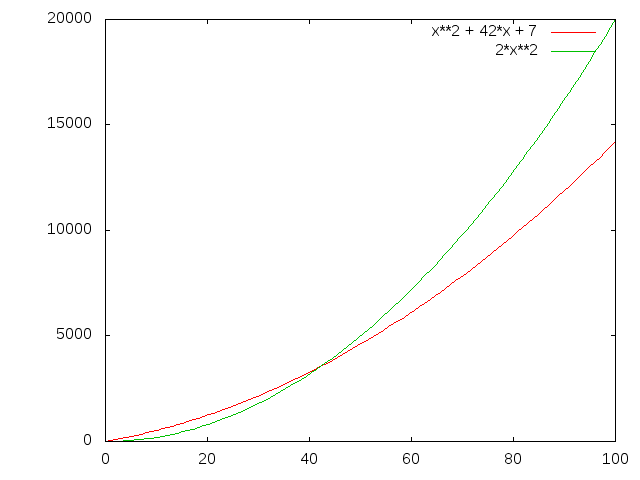
\includegraphics{figs/graph} \\[3ex]
    \begin{tabular}{c|cccccccccccc}
        &0&1&2&3&4&5&6&7&8&9&10&11 \\\hline
       0&0&1&0&0&1&0&0&0&0&0&0 &0\\
       1&1&0&1&0&0&1&1&0&0&0&0 &0\\
       2&1&0&0&1&0&0&1&0&0&0&0 &0\\
       3&0&0&1&0&0&0&0&1&0&0&0 &0\\
       4&1&0&0&0&0&1&0&0&1&0&0 &0\\
       5&0&1&1&0&1&0&1&0&0&1&0 &0\\
       6&0&0&1&0&0&1&0&1&0&0&1 &0\\
       7&0&0&0&1&0&0&1&0&0&0&0 &1\\
       8&0&0&0&0&1&0&0&0&0&1&0 &0\\
       9&0&0&0&0&0&1&0&0&1&0&1 &0\\
      10&0&0&0&0&0&0&1&0&0&1&0 &1\\
      11&0&0&0&0&0&0&0&1&0&0&1 &0\\
    \end{tabular} 
  \end{center}
  \caption{A graph and its adjacency matrix.}
  \figlabel{graph-adj}
\end{figure}

Where the adjacency matrix performs poorly is with the #outEdges(i)# and
#inEdges(i)# operations.  To implement these, we must scan all #n#
entries in the corresponding row or column of #a# and gather up all the
indices, #j#, where #a[i][j]#, respectively #a[j][i]#, is true.
\javaimport{ods/AdjacencyMatrix.outEdges(i).inEdges(i)}
\cppimport{ods/AdjacencyMatrix.outEdges(i,edges).inEdges(i,edges)}
These operations clearly take $O(#n#)$ time per operation.  

Another drawback of the adjacency matrix representation is that it
is big.  It stores an $#n#\times #n#$ boolean matrix, so it requires at
least $#n#^2$ bits of memory.  The implementation here uses a matrix
of \javaonly{#boolean#}\cpponly{#bool#} values so it actually uses on the
order of $#n#^2$ bytes of memory.  A more careful implementation, that
packs #w# boolean values into each word of memory could reduce this
space usage to $O(#n#^2/#w#)$ words of memory.

\begin{thm}
The #AdjacencyMatrix# data structure implements the #Graph# interface.
An #AdjacencyMatrix# supports the operations
\begin{itemize}
  \item #addEdge(i,j)#, #removeEdge(i,j)#, and #hasEdge(i,j)# in constant
  time per operation; and
  \item #inEdges(i)#, and #outEdges(i)# in $O(#n#)$ time per operation.
\end{itemize}
The space used by an #AdjacencyMatrix# is  $O(#n#^2)$.
\end{thm}

Despite the high memory usage and poor performance of the #inEdges(i)#
and #outEdges(i)# operations, an #AdjacencyMatrix# can still be useful for
some applications.  In particular, when the graph $G$ is \emph{dense},
i.e., it has close to $#n#^2$ edges, then a memory usage of $#n#^2$
may be acceptable.

The #AdjacencyMatrix# data structure is also commonly used because
algebraic operations on the matrix #a# can be used to efficiently compute
properties of the graph $G$.  This is a topic for a course on algorithms,
but we point out one such property here:  If we treat the entries of #a#
as integers (1 for #true# and 0 for #false#) and multiply #a# by itself
using matrix multiplication then we get the matrix $#a#^2$.  Recall,
from the definition of matrix multiplication, that
\[
    #a^2[i][j]# = \sum_{k=0}^{#n#-1} #a[i][k]#\cdot #a[k][j]# \enspace .
\]
Interpreting this sum in terms of the graph $G$, this formula counts the
number of vertices, $#k#$, such that $G$ contains both edges #(i,k)#
and #(k,j)#.  That is, it counts the number of paths from $#i#$ to $#j#$
(through intermediate vertices, $#k#$) that have length exactly 2.
This observation is the foundation of an algorithm that computes the
shortest paths between all pairs of vertices in $G$ using only $O(\log
#n#)$ matrix multiplications.

\section{#AdjacencyLists#: A Graph as a Collection of Lists}
\seclabel{adjacency-list}

\emph{Adjacency list} representations takes a more vertex-centric
approach.  There are many different possible implementations of
adjacency lists.  In this section, we present a simple one.  At the end
of the section, we discuss different possibilities.  In an adjacency
list representation, the graph $G=(V,E)$ is represented as an array,
#adj#, of lists.  The list #adj[i]# contains a list of all the vertices
adjacent to vertex #i#.  That is, it contains every index #j# such that
$#(i,j)#\in E$.
\codeimport{ods/AdjacencyLists.adj.n.AdjacencyLists(n0)}
(An example is shown in \figref{graph-adjlist}.)  In this particular
implementation, we represent each list in #adj# as \javaonly{an}\cpponly{a
subclass of} #ArrayStack#, because we would like constant time access
by position. Other options are also possible.  Specifically, we could
have implemented #adj# as a #DLList#.


\begin{figure}
  \begin{center}
    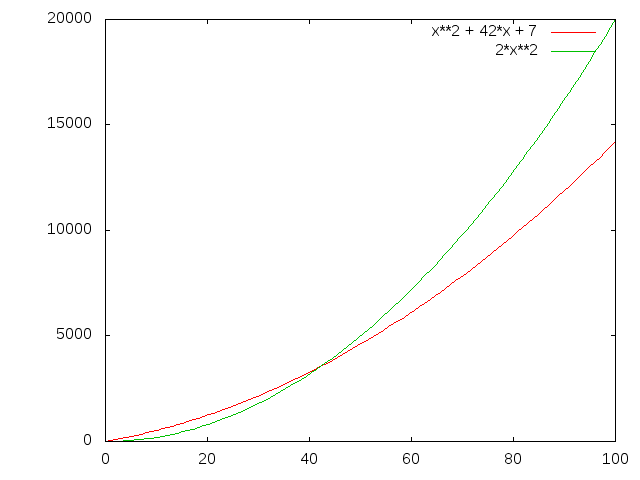
\includegraphics{figs/graph} \\[3ex]
    \begin{tabular}{|c|c|c|c|c|c|c|c|c|c|c|c|c|}\hline
        0&1&2&3&4&5&6 &7 &8&9 &10&11 \\\hline
        1&0&1&2&0&1&5 &6 &4&8 &9 &10 \\
        4&2&3&7&5&2&2 &3 &9&5 &6 &7 \\
         &6&6& &8&6&7 &11& &10&11& \\
         &5& & & &9&10&  & &  &  & \\
         & & & & &4&  &  & &  &  & \\
    \end{tabular} 
  \end{center}
  \caption{A graph and its adjacency lists}
  \figlabel{graph-adjlist}
\end{figure}



The #addEdge(i,j)# operation just appends the value #j# to the list #adj[i]#:
\codeimport{ods/AdjacencyLists.addEdge(i,j)}
This takes constant time.

The #removeEdge(i,j)# operation searches through the list #adj[i]#
until it finds #j# and then removes it:
\codeimport{ods/AdjacencyLists.removeEdge(i,j)}
This takes $O(\deg(#i#))$ time, where $\deg(#i#)$ (the \emph{degree} of
$#i#$) counts the number of edges in $E$ that have $#i#$ as their source.

The #hasEdge(i,j)# operation is similar;  it searches through the list
#adj[i]# until it finds #j# (and returns true), or reaches the end of
the list (and returns false):
\codeimport{ods/AdjacencyLists.hasEdge(i,j)}
This also takes $O(\deg(#i#))$ time.

The #outEdges(i)# operation is very simple;  \javaonly{It simply returns
the list #adj[i]#}\cpponly{It simply copies the values in #adj[i]#
into the output list}:
\javaimport{ods/AdjacencyLists.outEdges(i)}
\cppimport{ods/AdjacencyLists.outEdges(i,edges)}
\javaonly{This clearly takes constant time.}\cpponly{This clearly takes $O(\deg(#i#))$ time.}

The #inEdges(i)# operation is much more work.  It scans over every
vertex $j$ checking if the edge #(i,j)# exists and, if so, adding #j#
to the output list:
\javaimport{ods/AdjacencyLists.inEdges(i)}
\cppimport{ods/AdjacencyLists.inEdges(i,edges)}
This operation is very slow. It scans the adjacency list of every vertex,
so it takes $O(#n# + #m#)$ time.

The following theorem summarizes the performance of the above data structure:

\begin{thm}
The #AdjacencyLists# data structure implements the #Graph# interface.
An #AdjacencyLists# supports the operations
\begin{itemize}
  \item #addEdge(i,j)# in constant time per operation;
  \item #removeEdge(i,j)# and #hasEdge(i,j)# in $O(\deg(#i#))$ time
    per operation;
  \javaonly{\item #outEdges(i)# in constant time per operation; and}
  \cpponly{\item #outEdges(i)# in $O(\deg(#i#))$ time per operation; and}
  \item #inEdges(i)# in $O(#n#+#m#)$ time per operation.
\end{itemize}
The space used by a #AdjacencyLists# is  $O(#n#+#m#)$.
\end{thm}

As alluded to earlier, there are many different choices to be made when
implementing a graph as an adjacency list.  Some questions that come
up include:
\begin{itemize}
  \item What type of collection should be used to store each element
  of #adj#?  One could use an array-based list,  a linked-list, or even
  a hashtable.
  \item Should there be a second adjacency list, #inadj#, that stores,
  for each #i#, the list of vertices, #j#, such that $#(j,i)#\in E$?
  This can greatly reduce the running-time of the #inEdges(i)#
  operation, but requires slightly more work when adding or removing
  edges.
  \item Should the entry for the edge #(i,j)# in #adj[i]# be linked by
  a reference to the corresponding entry in #inadj[j]#?
  \item Should edges be first-class objects with their own associated data?
  In this way, #adj# would contain lists of edges rather than lists of vertices (integers).
\end{itemize}
Most of these questions come down to a tradeoff between complexity (and
space) of implementation and performance features of the implementation.

\section{Graph Traversal}

In this section we present two algorithms for exploring a graph, starting
at one of its vertices, #i#, and finding all vertices that are reachable
from #i#.  Both of these algorithms are best suited to graphs represented
using an adjacency list representation.  Therefore, when analyzing these
algorithms we will assume that the underlying representation is as an
#AdjacencyLists#.

\subsection{Breadth-First Search}

The \emph{bread-first-search} algorithm starts at a vertex #i# and visits,
first the neighbours of #i#, then the neighbours of the neighbours of #i#,
then the neighbours of the neighbours of the neighbours of #i#, and so on.

This algorithm is a generalization of the breadth-first-search algorithm
for binary trees (\secref{bintree:traversal}), and is very similar; it
uses a queue, #q#, that initially contains only #i#.  It then repeatedly
extracts an element from #q# and adds its neighbours to #q#, provided
that these neighbours have never been in #q# before.  The only major difference
between breadth-first-search for graphs and for trees
is that the algorithm for graphs has to ensure that it does not
add the same vertex to #q# more than once.  It does this by using an
auxiliary boolean array, #seen#, that keeps track of which vertices have
already been discovered.
\codeimport{ods/Algorithms.bfs(g,r)}
An example of running #bfs(g,0)# on the graph from \figref{graph}
is shown in \figref{graph-bfs}.  Different executions are possible,
depending on the ordering of the adjacency lists; \figref{graph-bfs}
uses the adjacency lists in \figref{graph-adjlist}.

\begin{figure}
  \begin{center}
    \includegraphics{figs/graph-bfs}
  \end{center}
  \caption[Breadth-first-search]{An example of bread-first-search starting at node 0. Nodes are
  labelled with the order in which they are added to #q#.  Edges that
  result in nodes being added to #q# are drawn in black, other edges
  are drawn in grey.}
  \figlabel{graph-bfs}
\end{figure}

Analyzing the running-time of the #bfs(g,i)# routine is fairly
straightforward.  The use of the #seen# array ensures that no vertex is
added to #q# more than once.  Adding (and later removing) each vertex
from #q# takes constant time per vertex for a total of $O(#n#)$ time.
Since each vertex is processed at most once by the inner loop, each
adjacency list is processed at most once, so each edge of $G$ is processed
at most once.  This processing, which is done in the inner loop takes
constant time per iteration, for a total of $O(#m#)$ time.  Therefore,
the entire algorithm runs in $O(#n#+#m#)$ time.

The following theorem summarizes the performance of the #bfs(g,r)# algorithm.
\begin{thm}\thmlabel{bfs-graph}
  When given as input a #Graph#, #g#, that is implemented using the
  #AdjacencyLists# data structure, the #bfs(g,r)# algorithm runs in $O(#n#+#m#)$
  time.
\end{thm}

A breadth-first traversal has some very special properties.  Calling
#bfs(g,r)# will eventually enqueue (and eventually dequeue) every vertex
#j# such that there is a directed path from #r# to #j#.  Moreover,
the vertices at distance 0 from #r# (#r# itself) will enter #q# before
the vertices at distance 1, which will enter #q# before the vertices at
distance 2, and so on.  Thus, the #bfs(g,r)# method visits vertices
in increasing order of distance from #r# and vertices that can not be
reached from #r# are never output at all.

A particularly useful application of the breadth-first-search algorithm
is, therefore, in computing shortest paths.  To compute the shortest
path from #r# to every other vertex, we use a variant of #bfs(g,r)#
that uses an auxilliary array, #p#, of length #n#.  When a new vertex
#j# is added to #q#, we set #p[j]=i#.  In this way, #p[j]# becomes the
second last node on a shortest path from #r# to #j#.  Repeating this,
by taking #p[p[j]#, #p[p[p[j]]]#, and so on we can reconstruct the
(reversal of) a shortest path from #r# to #j#.



\subsection{Depth-First Search}

The \emph{depth-first-search} algorithm is similar to the standard
algorithm for traversing binary trees;  it first fully explores one
subtree before returning to the current node and then exploring the
other subtree.  Another way to think of depth-first-search is by saying
that it is similar to breadth-first search except that it uses a stack
instead of a queue.

During the execution of the depth-first-search algorithm, each vertex,
#i#, is assigned a color, #c[i]#: #white# if we have never seen
the vertex before, #grey# if we are currently visiting that vertex,
and #black# if we are done visiting that vertex.  The easiest way to
think of depth-first-search is as a recursive algorithm.  It starts by
visiting #r#.  When visiting a vertex #i#, we first mark #i# as #grey#.
Next, we scan #i#'s adjacency list and recursively visit any white vertex
we find in this list.  Finally, we are done processing #i#, so we color
#i# black and return.
\codeimport{ods/Algorithms.dfs(g,r).dfs(g,i,c)}
An example of the execution of this algorithm is shown in \figref{graph-dfs}

\begin{figure}
  \begin{center}
    \includegraphics{figs/graph-dfs}
  \end{center}
  \caption[Depth-first-search]{An example of depth-first-search starting at node 0. Nodes are
  labelled with the order in which they are processed.  Edges that
  result in a recursive call are drawn in black, other edges
  are drawn in #grey#.}
  \figlabel{graph-dfs}
\end{figure}

Although depth-first-search may best be thought of as a recursive
algorithm, recursion is not the best way to implement it. Indeed, the code
given above will fail for many large graphs by causing a stack overflow.
An alternative implementation is to replace the recursion stack with an
explicit stack, #s#.  The following implementation does just that:
\codeimport{ods/Algorithms.dfs2(g,r)} 
In the above code, when next vertex, #i#, is processed, #i# is colored
#grey# and then replaced, on the stack, with its adjacent vertices.
During the next iteration, one of these vertices will be visited.

Not surprisingly, the running times of #dfs(g,r)# and #dfs2(g,r)# are the
same as that of #bfs(g,r)#:
\begin{thm}\thmlabel{dfs-graph}
  When given as input a #Graph#, #g#, that is implemented using the
  #AdjacencyLists# data structure, the #dfs(g,r)# and #dfs2(g,r)# algorithms
  each run in $O(#n#+#m#)$ time.
\end{thm}

As with the breadth-first-search algorithm, there is an underlying
tree associated with each execution of depth-first-search.  When a node
$#i#\neq #r#$ goes from #white# to #grey#, this is because #dfs(g,i,c)#
was called recursively while processing some node #i'#.  (In the case
of #dfs2(g,r)# algorithm, #i# is one of the nodes that replaced #i'#
on the stack.)  If we think of #i'# as the parent of #i#, then we obtain
a tree rooted at #r#.  In \figref{graph-dfs}, this tree is a path from
vertex 0 to vertex 11.

An important property of the depth-first-search algorithm is the
following: Suppose that when node #i# is colored #grey#, there exists a path
from #i# to some other node #j# that uses only white vertices.  Then #j#
will be colored (first #grey# then) #black# before #i# is colored #black#.
(This can be proven by contradiction, by considering any path $P$ from #i#
to #j#.)

One application of this property is the detection of cycles. Refer
to \figref{dfs-cycle}.  Consider some cycle, $C$, that can be reached
from #r#.  Let #i# be the first node of $C$ that is colored #grey#,
and let #j# be the node that precedes #i# on the cycle $C$.  Then,
by the above property, #j# will be colored #grey# and the edge #(j,i)#
will be considered by the algorithm while #i# is still #grey#.  Thus,
the algorithm can conclude that there is a path, $P$, from #i# to #j#
in the depth-first-search tree and the edge #(j,i)# exists.  Therefore,
$P$ is also a cycle.

\begin{figure}
  \begin{center}
    \includegraphics{figs/dfs-cycle}
  \end{center}
  \caption[Cycle detection]{The depth-first-search algorithm can be used to detect cycles
  in $G$.The node #j# is colored #grey# while #i# is still #grey#.  This
  implies there is a path, $P$, from #i# to #j# in the depth-first-search
  tree, and the edge #(j,i)# implies that $P$ is also a cycle.}
  \figlabel{dfs-cycle}
\end{figure}

\section{Discussion and Exercises}

The running times of the depth-first-search and breadth-first-search
algorithms are somewhat overstated by the Theorems~\ref{thm:bfs-graph} and
\ref{thm:dfs-graph}.  Define $#n#_{#r#}$ as the number of vertices, #i#,
of $G$, for which there exists a path from #r# to #i#.  Define $#m#_#r#$
as the number of edges that have these vertices as their sources.
Then the following theorem is a more precise statement of the running
times of the breadth-first-search and depth-first-search algorithms.
(This more refined statement of the running time is useful in some of
the applications of these algorithms outlined in the exercises.)
\begin{thm}\thmlabel{graph-traversal}
  When given as input a #Graph#, #g#, that is implemented using the
  #AdjacencyLists# data structure, the #bfs(g,r)#, #dfs(g,r)# and #dfs2(g,r)#
  algorithms each run in $O(#n#_{#r#}+#m#_{#r#})$ time.
\end{thm}

Breadth-first search seems to have been discovered independently by
Moore \cite{m59} and Lee \cite{l61} in the contexts of maze exploration
and circuit routing, respectively.

Adjacency-list representations of graphs were first popularized by
Hopcroft and Tarjan \cite{ht73} as an alternative to the (then more
common) adjacency-matrix representation.  This representation, and
depth-first-search, played a major part in the celebrated Hopcroft-Tarjan
planarity testing algorithm that can determine, in $O(#n#)$ time, if
a graph can be drawn, in the plane, and in such a way that no pair of
edges cross each other \cite{ht74}.

In the following exercises, an undirected graph is one in which, for
every #i# and #j#, the edge $(#i#,#j#)$ is present if and only if the
edge $(#j#,#i#)$ is present.

\begin{exc}
  Draw an adjacencly list representation and an adjacency matrix
  representation of the graph in \figref{graph-example2}.
\end{exc}

\begin{figure}
  \centering{\includegraphics{figs/graph-example2}}
  \caption{An example graph.}
  \figlabel{graph-example2}
\end{figure}

\begin{exc}
  The \emph{incidence matrix} representation of a graph,
  $G$, is an $#n#\times#m#$ matrix, $A$, where
  \[
     A_{i,j} = \begin{cases}
        -1 & \text{if vertex $i$ the source of edge $j$} \\
        +1 & \text{if vertex $i$ the target of edge $j$} \\
        0 & \text{otherwise.}
     \end{cases}
  \]
  \begin{enumerate}
    \item Draw the incident matrix representation of the graph in
      \figref{graph-example2}.
    \item Design, analyze and implement an incidence matrix representation
      of a graph.  Be sure to analyze the space, the cost of
      #addEdge(i,j)#, #removeEdge(i,j)#, #hasEdge(i,j)#, #inEdges(i)#,
      and #outEdges(i)#.
  \end{enumerate}
\end{exc}

\begin{exc}
  Illustrate an execution of the #bfs(G,0)# and #dfs(G,0)# on the graph, $#G#$,
  in \figref{graph-example2}.
\end{exc}

\begin{exc}
  Let $G$ be an undirected graph.  We say $G$ is \emph{connected} if,
  for every pair of vertices #i# and #j# in $G$, there is a path from
  $#i#$ to $#j#$ (since $G$ is undirected, there is also a path from #j#
  to #i#). Show how to test if $G$ is connected in $O(#n#+#m#)$ time.
\end{exc}

\begin{exc}
  Let $G$ be an undirected graph.  A \emph{connected-component labelling}
  of $G$ partitions the vertices of $G$ into maximal sets, each of which
  forms a connected subgraph.  Show how to compute a connected component
  labelling of $G$ in $O(#n#+#m#)$ time.
\end{exc}

\begin{exc}
  Let $G$ be an undirected graph.  A \emph{spanning forest} of $G$ is a
  collection of trees, one per component, whose edges are edges of $G$
  and whose vertices contain all vertices of $G$.  Show how to compute
  a spanning forest of of $G$ in $O(#n#+#m#)$ time.
\end{exc}

\begin{exc}
  We say that a graph $G$ is \emph{strongly-connected} if, for every
  pair of vertices #i# and #j# in $G$, there is a path from $#i#$ to
  $#j#$. Show how to test if $G$ is strongly-connected in $O(#n#+#m#)$
  time.
\end{exc}

\begin{exc}
  Given a graph $G=(V,E)$ and some special vertex $#r#\in V$, show how
  to compute the length of the shortest path from $#r#$ to #i# for every
  vertex $#i#\in V$.
\end{exc}

\begin{exc}
  Give a (simple) example where the #dfs(g,r)# code visits the nodes of a
  graph in an order that is different from that of the #dfs2(g,r)# code.
  Write a version of #dfs2(g,r)# that always visits nodes in exactly
  the same order as #dfs(g,r)#.  (Hint: Just start tracing the execution
  of each algorithm on some graph where #r# is the source of more than
  1 edge.)
\end{exc}

\begin{exc}
  A \emph{universal sink} in a graph $G$ is a vertex that is the target
  of $#n#-1$ edges and the source of no edges.\footnote{A universal sink,
  #v#, is also sometimes called a \emph{celebrity}: Everyone in the room
  recognizes #v#, but #v# doesn't recognize anyone else in the room.}
  Design and implement an algorithm that tests if a graph $G$, represented
  as an #AdjacencyMatrix#, has a universal sink.  Your algorithm should
  run in $O(#n#)$ time.
\end{exc}



